\documentclass{whiteboard}
\begin{document}
\begin{frame}[plain,t]
 \bbcover{Grafos}{Componentes Conectados}{Prof. Edson Alves}{Faculdade UnB Gama}
\end{frame}

\begin{frame}[plain,t]
\begin{tikzpicture}
\node[draw,opacity=0] at (0, 0) {x};
\node[draw,opacity=0] at (14, 8) {x};
 \node[anchor=west] at (0, 6) { \Large \bbbold{Grafos conectados} };
\end{tikzpicture}
\end{frame}

\begin{frame}[plain,t]
\begin{tikzpicture}
\node[draw,opacity=0] at (0, 0) {x};
\node[draw,opacity=0] at (14, 8) {x};
 \node[anchor=west] at (0, 6) { \Large \bbbold{Grafos conectados} };
 \node[anchor=west] at (1, 5) { \bbtext{Um grafo não-direcionado $G(V, E)$ é dito \bbbold{conectado} se, para qualquer} };
\end{tikzpicture}
\end{frame}

\begin{frame}[plain,t]
\begin{tikzpicture}
\node[draw,opacity=0] at (0, 0) {x};
\node[draw,opacity=0] at (14, 8) {x};
 \node[anchor=west] at (0, 6) { \Large \bbbold{Grafos conectados} };
 \node[anchor=west] at (1, 5) { \bbtext{Um grafo não-direcionado $G(V, E)$ é dito \bbbold{conectado} se, para qualquer} };
 \node[anchor=west] at (0.5, 4) { \bbtext{par de vértices $u, v\in V$, existe ao menos um caminho de $u$ a $v$.} };
\end{tikzpicture}
\end{frame}

\begin{frame}[plain,t]
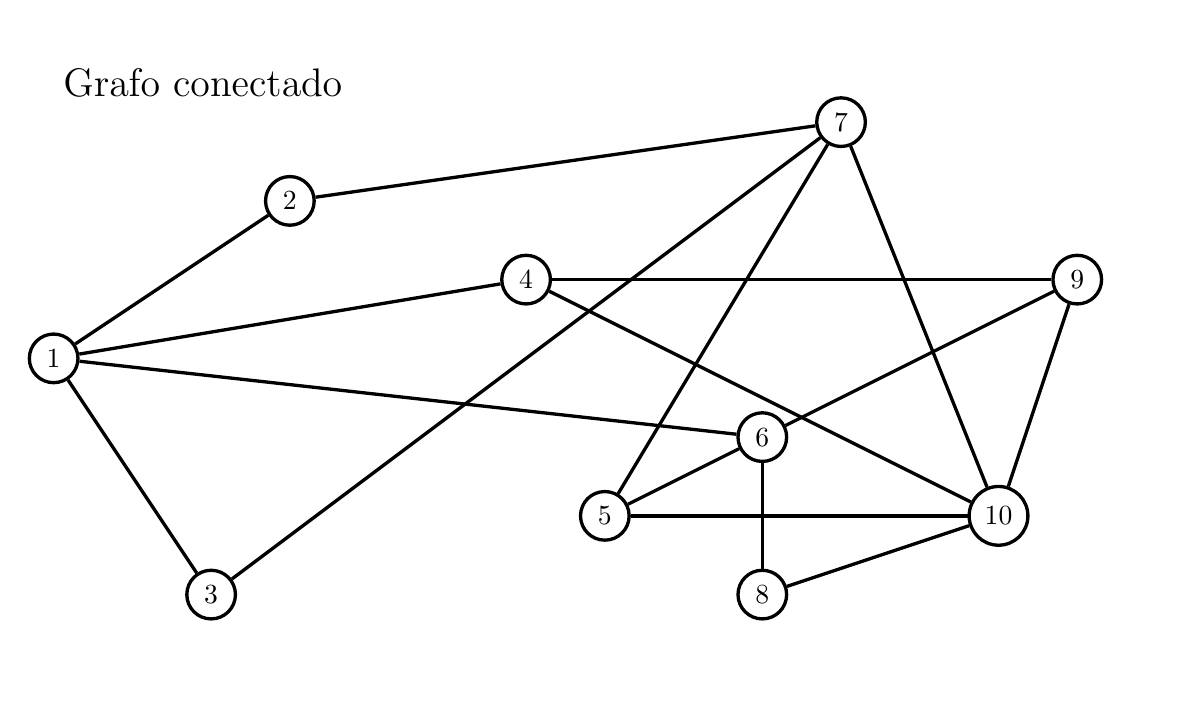
\begin{tikzpicture}
\node[draw,opacity=0] at (0, 0) {x};
\node[draw,opacity=0] at (14, 8) {x};
 \node[anchor=west] at (0, 7.5) { \Large \bbbold{Grafo conectado} };
 \node[circle,draw,very thick] (A) at (0, 4) {\bbtext{1}};
 \node[circle,draw,very thick] (B) at (3, 6) {\bbtext{2}};
 \node[circle,draw,very thick] (C) at (2, 1) {\bbtext{3}};
 \node[circle,draw,very thick] (D) at (6, 5) {\bbtext{4}};
 \node[circle,draw,very thick] (E) at (7, 2) {\bbtext{5}};
 \node[circle,draw,very thick] (F) at (9, 3) {\bbtext{6}};
 \node[circle,draw,very thick] (G) at (10, 7) {\bbtext{7}};
 \node[circle,draw,very thick] (H) at (9, 1) {\bbtext{8}};
 \node[circle,draw,very thick] (I) at (13, 5) {\bbtext{9}};
 \node[circle,draw,very thick] (J) at (12, 2) {\bbtext{10}};
 \draw[very thick] (A) -- (B);
 \draw[very thick] (A) -- (C);
 \draw[very thick] (A) -- (D);
 \draw[,very thick] (A) -- (F);
 \draw[very thick] (B) -- (G);
 \draw[very thick] (C) -- (G);
 \draw[very thick] (D) -- (I);
 \draw[very thick] (D) -- (J);
 \draw[very thick] (E) -- (F);
 \draw[very thick] (E) -- (G);
 \draw[very thick] (E) -- (J);
 \draw[very thick] (F) -- (H);
 \draw[very thick] (F) -- (I);
 \draw[very thick] (G) -- (J);
 \draw[very thick] (H) -- (J);
 \draw[very thick] (I) -- (J);
\end{tikzpicture}
\end{frame}

\begin{frame}[plain,t]
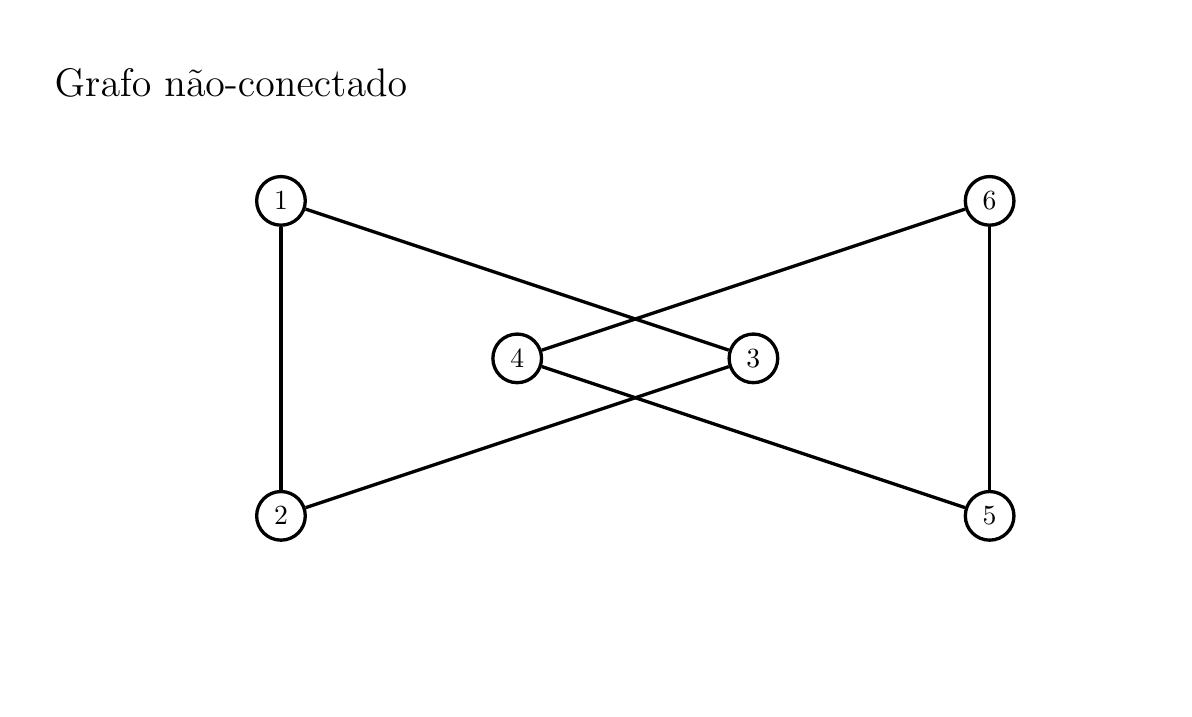
\begin{tikzpicture}
\node[draw,opacity=0] at (0, 0) {x};
\node[draw,opacity=0] at (14, 8) {x};
 \node[anchor=west] at (0, 7.5) { \Large \bbbold{Grafo não-conectado} };
 \node[circle,draw,very thick] (A) at (3, 6) {\bbtext{1}};
 \node[circle,draw,very thick] (B) at (3, 2) {\bbtext{2}};
 \node[circle,draw,very thick] (C) at (9, 4) {\bbtext{3}};
 \node[circle,draw,very thick] (D) at (6, 4) {\bbtext{4}};
 \node[circle,draw,very thick] (E) at (12, 2) {\bbtext{5}};
 \node[circle,draw,very thick] (F) at (12, 6) {\bbtext{6}};
 \draw[very thick] (A) -- (B);
 \draw[very thick] (A) -- (C);
 \draw[very thick] (B) -- (C);
 \draw[very thick] (D) -- (E);
 \draw[very thick] (D) -- (F);
 \draw[very thick] (E) -- (F);
\end{tikzpicture}
\end{frame}

\begin{frame}[plain,t]
\begin{tikzpicture}
\node[draw,opacity=0] at (0, 0) {x};
\node[draw,opacity=0] at (14, 8) {x};
 \node[anchor=west] at (0, 7) { \Large \bbbold{Componente conectado} };
\end{tikzpicture}
\end{frame}

\begin{frame}[plain,t]
\begin{tikzpicture}
\node[draw,opacity=0] at (0, 0) {x};
\node[draw,opacity=0] at (14, 8) {x};
 \node[anchor=west] at (0, 7) { \Large \bbbold{Componente conectado} };
 \node[anchor=west] at (1, 6) { \bbtext{O componente conectado do grafo $G(V,E)$ que contém o vértice $u$ é o maior} };
 \node[anchor=west] at (0.5, 5) { \bbtext{subgrafo conectado $S(V', E')$ de $G$ tal que $v\in V'$ } };
\end{tikzpicture}
\end{frame}

\begin{frame}[plain,t]
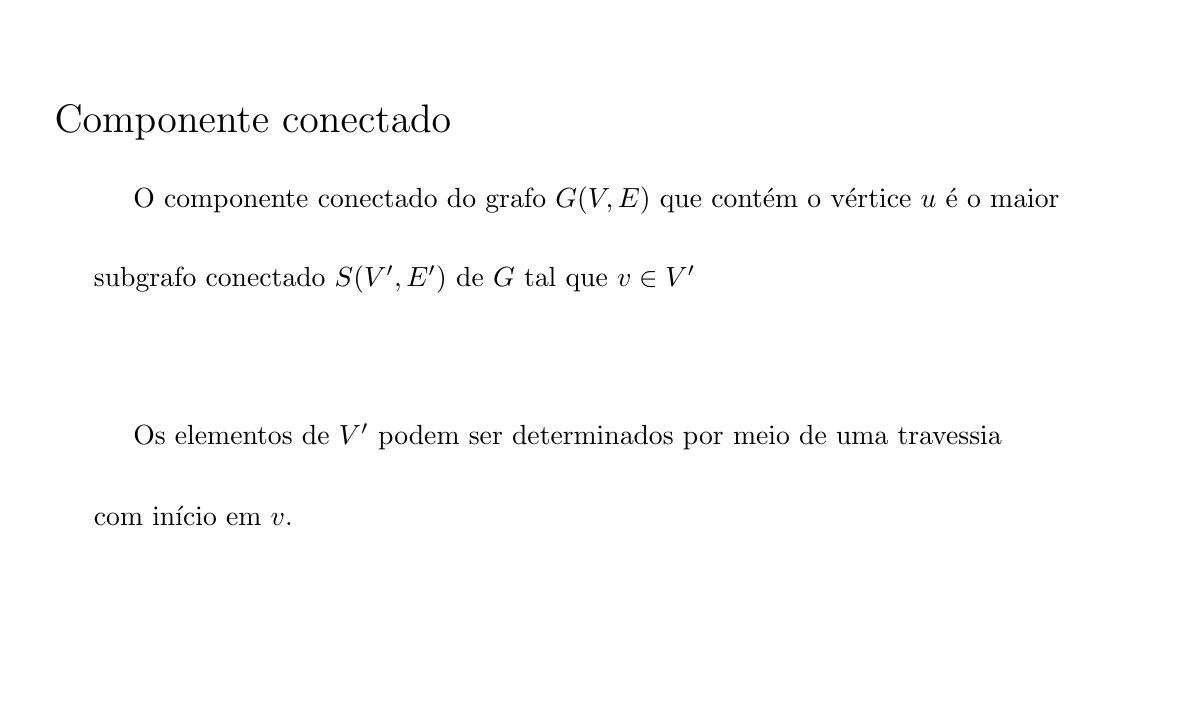
\begin{tikzpicture}
\node[draw,opacity=0] at (0, 0) {x};
\node[draw,opacity=0] at (14, 8) {x};
 \node[anchor=west] at (0, 7) { \Large \bbbold{Componente conectado} };
 \node[anchor=west] at (1, 6) { \bbtext{O componente conectado do grafo $G(V,E)$ que contém o vértice $u$ é o maior} };
 \node[anchor=west] at (0.5, 5) { \bbtext{subgrafo conectado $S(V', E')$ de $G$ tal que $v\in V'$ } };
 \node[anchor=west] at (1, 3) { \bbtext{Os elementos de $V'$ podem ser determinados por meio de uma travessia} };
 \node[anchor=west] at (0.5, 2) { \bbtext{com início em $v$. } };
\end{tikzpicture}
\end{frame}

\begin{frame}[plain,t]
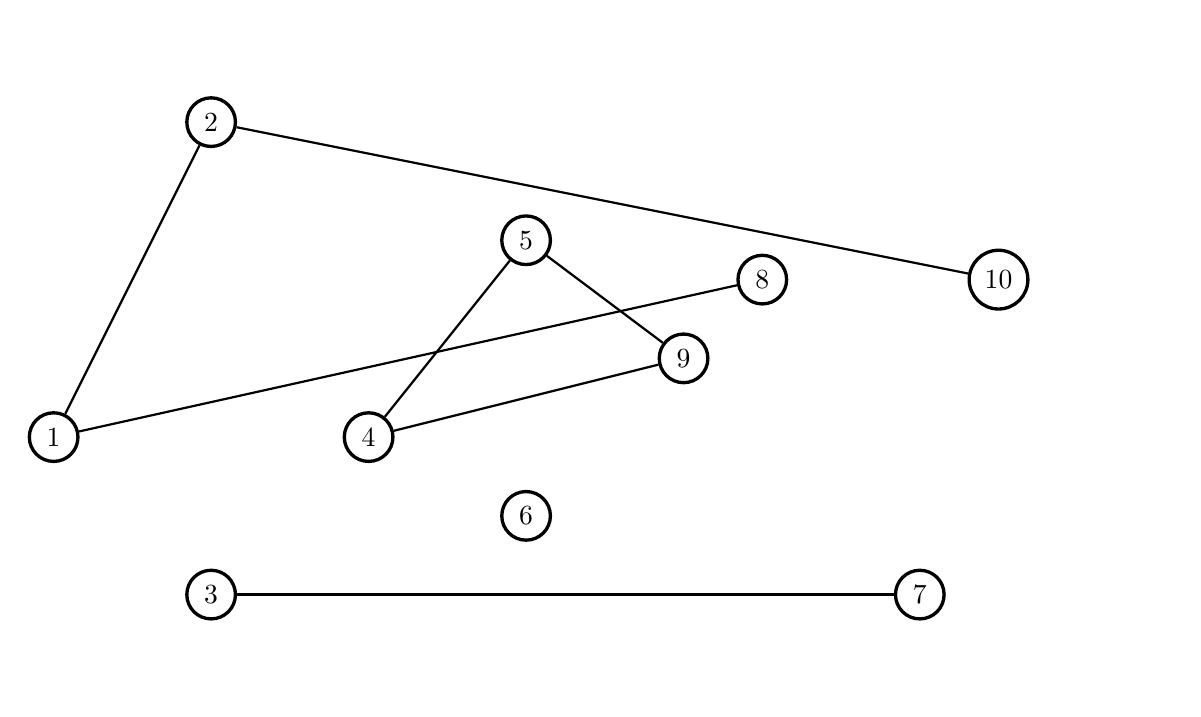
\begin{tikzpicture}
\node[draw,opacity=0] at (0, 0) {x};
\node[draw,opacity=0] at (14, 8) {x};
 \node[circle, draw, very thick] (A) at (0, 3) { \bbtext{1} };
 \node[circle, draw, very thick] (B) at (2, 7) { \bbtext{2} };
 \node[circle, draw, very thick] (C) at (2, 1) { \bbtext{3} };
 \node[circle, draw, very thick] (D) at (4, 3) { \bbtext{4} };
 \node[circle, draw, very thick] (E) at (6, 5.5) { \bbtext{5} };
 \node[circle, draw, very thick] (F) at (6, 2) { \bbtext{6} };
 \node[circle, draw, very thick] (G) at (11, 1) { \bbtext{7} };
 \node[circle, draw, very thick] (H) at (9, 5) { \bbtext{8} };
 \node[circle, draw, very thick] (I) at (8, 4) { \bbtext{9} };
 \node[circle, draw, very thick] (J) at (12, 5) { \bbtext{10} };
 \draw[thick] (A) to (B);
 \draw[thick] (A) to (H);
 \draw[thick] (B) to (J);
 \draw[thick] (D) to (E);
 \draw[thick] (D) to (I);
 \draw[thick] (E) to (I);
 \draw[thick] (C) to (G);
\end{tikzpicture}
\end{frame}

\begin{frame}[plain,t]
\begin{tikzpicture}
\node[draw,opacity=0] at (0, 0) {x};
\node[draw,opacity=0] at (14, 8) {x};
 \node[circle, draw, very thick] (B) at (2, 7) { \bbtext{2} };
 \node[circle, draw, very thick] (C) at (2, 1) { \bbtext{3} };
 \node[circle, draw, very thick] (D) at (4, 3) { \bbtext{4} };
 \node[circle, draw, very thick] (E) at (6, 5.5) { \bbtext{5} };
 \node[circle, draw, very thick] (F) at (6, 2) { \bbtext{6} };
 \node[circle, draw, very thick] (G) at (11, 1) { \bbtext{7} };
 \node[circle, draw, very thick] (H) at (9, 5) { \bbtext{8} };
 \node[circle, draw, very thick] (I) at (8, 4) { \bbtext{9} };
 \node[circle, draw, very thick] (J) at (12, 5) { \bbtext{10} };
 \draw[thick] (A) to (B);
 \draw[thick] (A) to (H);
 \draw[thick] (B) to (J);
 \draw[thick] (D) to (E);
 \draw[thick] (D) to (I);
 \draw[thick] (E) to (I);
 \draw[thick] (C) to (G);
 \node[circle, fill, color=BBCyan] (A) at (0, 3) { \bbtext{1} };
 \node[circle, draw, very thick] (A) at (0, 3) { \bbtext{1} };
\end{tikzpicture}
\end{frame}

\begin{frame}[plain,t]
\begin{tikzpicture}
\node[draw,opacity=0] at (0, 0) {x};
\node[draw,opacity=0] at (14, 8) {x};
 \node[circle, draw, very thick] (C) at (2, 1) { \bbtext{3} };
 \node[circle, draw, very thick] (D) at (4, 3) { \bbtext{4} };
 \node[circle, draw, very thick] (E) at (6, 5.5) { \bbtext{5} };
 \node[circle, draw, very thick] (F) at (6, 2) { \bbtext{6} };
 \node[circle, draw, very thick] (G) at (11, 1) { \bbtext{7} };
 \node[circle, draw, very thick] (H) at (9, 5) { \bbtext{8} };
 \node[circle, draw, very thick] (I) at (8, 4) { \bbtext{9} };
 \node[circle, draw, very thick] (J) at (12, 5) { \bbtext{10} };
 \draw[thick] (A) to (H);
 \draw[thick] (B) to (J);
 \draw[thick] (D) to (E);
 \draw[thick] (D) to (I);
 \draw[thick] (E) to (I);
 \draw[thick] (C) to (G);
 \node[circle, fill, color=BBCyan] (A) at (0, 3) { \bbtext{1} };
 \node[circle, draw, very thick] (A) at (0, 3) { \bbtext{1} };
 \node[circle, fill, color=BBCyan] (B) at (2, 7) { \bbtext{2} };
 \node[circle, draw, very thick] (B) at (2, 7) { \bbtext{2} };
 \draw[-latex,very thick] (A) to (B);
\end{tikzpicture}
\end{frame}

\begin{frame}[plain,t]
\begin{tikzpicture}
\node[draw,opacity=0] at (0, 0) {x};
\node[draw,opacity=0] at (14, 8) {x};
 \node[circle, draw, very thick] (C) at (2, 1) { \bbtext{3} };
 \node[circle, draw, very thick] (D) at (4, 3) { \bbtext{4} };
 \node[circle, draw, very thick] (E) at (6, 5.5) { \bbtext{5} };
 \node[circle, draw, very thick] (F) at (6, 2) { \bbtext{6} };
 \node[circle, draw, very thick] (G) at (11, 1) { \bbtext{7} };
 \node[circle, draw, very thick] (H) at (9, 5) { \bbtext{8} };
 \node[circle, draw, very thick] (I) at (8, 4) { \bbtext{9} };
 \draw[thick] (A) to (H);
 \draw[thick] (D) to (E);
 \draw[thick] (D) to (I);
 \draw[thick] (E) to (I);
 \draw[thick] (C) to (G);
 \node[circle, fill, color=BBCyan] (A) at (0, 3) { \bbtext{1} };
 \node[circle, draw, very thick] (A) at (0, 3) { \bbtext{1} };
 \node[circle, fill, color=BBCyan] (B) at (2, 7) { \bbtext{2} };
 \node[circle, draw, very thick] (B) at (2, 7) { \bbtext{2} };
 \draw[-latex,very thick] (A) to (B);
 \node[circle, fill, color=BBCyan] (J) at (12, 5) { \bbtext{10} };
 \node[circle, draw, very thick] (J) at (12, 5) { \bbtext{10} };
 \draw[-latex, very thick] (B) to (J);
\end{tikzpicture}
\end{frame}

\begin{frame}[plain,t]
\begin{tikzpicture}
\node[draw,opacity=0] at (0, 0) {x};
\node[draw,opacity=0] at (14, 8) {x};
 \node[circle, draw, very thick] (C) at (2, 1) { \bbtext{3} };
 \node[circle, draw, very thick] (D) at (4, 3) { \bbtext{4} };
 \node[circle, draw, very thick] (E) at (6, 5.5) { \bbtext{5} };
 \node[circle, draw, very thick] (F) at (6, 2) { \bbtext{6} };
 \node[circle, draw, very thick] (G) at (11, 1) { \bbtext{7} };
 \node[circle, draw, very thick] (I) at (8, 4) { \bbtext{9} };
 \draw[thick] (D) to (E);
 \draw[thick] (D) to (I);
 \draw[thick] (E) to (I);
 \draw[thick] (C) to (G);
 \node[circle, fill, color=BBCyan] (A) at (0, 3) { \bbtext{1} };
 \node[circle, draw, very thick] (A) at (0, 3) { \bbtext{1} };
 \node[circle, fill, color=BBCyan] (B) at (2, 7) { \bbtext{2} };
 \node[circle, draw, very thick] (B) at (2, 7) { \bbtext{2} };
 \draw[-latex,very thick] (A) to (B);
 \node[circle, fill, color=BBCyan] (J) at (12, 5) { \bbtext{10} };
 \node[circle, draw, very thick] (J) at (12, 5) { \bbtext{10} };
 \draw[-latex, very thick] (B) to (J);
 \node[circle, fill, color=BBCyan] (H) at (9, 5) { \bbtext{8} };
 \node[circle, draw, very thick] (H) at (9, 5) { \bbtext{8} };
 \draw[-latex,very thick] (A) to (H);
\end{tikzpicture}
\end{frame}

\begin{frame}[plain,t]
\begin{tikzpicture}
\node[draw,opacity=0] at (0, 0) {x};
\node[draw,opacity=0] at (14, 8) {x};
 \node[circle, draw, very thick] (C) at (2, 1) { \bbtext{3} };
 \node[circle, draw, very thick] (E) at (6, 5.5) { \bbtext{5} };
 \node[circle, draw, very thick] (F) at (6, 2) { \bbtext{6} };
 \node[circle, draw, very thick] (G) at (11, 1) { \bbtext{7} };
 \node[circle, draw, very thick] (I) at (8, 4) { \bbtext{9} };
 \draw[thick] (D) to (E);
 \draw[thick] (D) to (I);
 \draw[thick] (E) to (I);
 \draw[thick] (C) to (G);
 \node[circle, fill, color=BBCyan] (A) at (0, 3) { \bbtext{1} };
 \node[circle, draw, very thick] (A) at (0, 3) { \bbtext{1} };
 \node[circle, fill, color=BBCyan] (B) at (2, 7) { \bbtext{2} };
 \node[circle, draw, very thick] (B) at (2, 7) { \bbtext{2} };
 \draw[-latex,very thick] (A) to (B);
 \node[circle, fill, color=BBCyan] (J) at (12, 5) { \bbtext{10} };
 \node[circle, draw, very thick] (J) at (12, 5) { \bbtext{10} };
 \draw[-latex, very thick] (B) to (J);
 \node[circle, fill, color=BBCyan] (H) at (9, 5) { \bbtext{8} };
 \node[circle, draw, very thick] (H) at (9, 5) { \bbtext{8} };
 \draw[-latex,very thick] (A) to (H);
 \node[circle, fill, color=BBOrange] (D) at (4, 3) { \bbtext{4} };
 \node[circle, draw, very thick] (D) at (4, 3) { \bbtext{4} };
\end{tikzpicture}
\end{frame}

\begin{frame}[plain,t]
\begin{tikzpicture}
\node[draw,opacity=0] at (0, 0) {x};
\node[draw,opacity=0] at (14, 8) {x};
 \node[circle, draw, very thick] (C) at (2, 1) { \bbtext{3} };
 \node[circle, draw, very thick] (F) at (6, 2) { \bbtext{6} };
 \node[circle, draw, very thick] (G) at (11, 1) { \bbtext{7} };
 \node[circle, draw, very thick] (I) at (8, 4) { \bbtext{9} };
 \draw[thick] (D) to (I);
 \draw[thick] (E) to (I);
 \draw[thick] (C) to (G);
 \node[circle, fill, color=BBCyan] (A) at (0, 3) { \bbtext{1} };
 \node[circle, draw, very thick] (A) at (0, 3) { \bbtext{1} };
 \node[circle, fill, color=BBCyan] (B) at (2, 7) { \bbtext{2} };
 \node[circle, draw, very thick] (B) at (2, 7) { \bbtext{2} };
 \draw[-latex,very thick] (A) to (B);
 \node[circle, fill, color=BBCyan] (J) at (12, 5) { \bbtext{10} };
 \node[circle, draw, very thick] (J) at (12, 5) { \bbtext{10} };
 \draw[-latex, very thick] (B) to (J);
 \node[circle, fill, color=BBCyan] (H) at (9, 5) { \bbtext{8} };
 \node[circle, draw, very thick] (H) at (9, 5) { \bbtext{8} };
 \draw[-latex,very thick] (A) to (H);
 \node[circle, fill, color=BBOrange] (D) at (4, 3) { \bbtext{4} };
 \node[circle, draw, very thick] (D) at (4, 3) { \bbtext{4} };
 \node[circle, fill, color=BBOrange] (E) at (6, 5.5) { \bbtext{5} };
 \node[circle, draw, very thick] (E) at (6, 5.5) { \bbtext{5} };
 \draw[-latex,very thick] (D) to (E);
\end{tikzpicture}
\end{frame}

\begin{frame}[plain,t]
\begin{tikzpicture}
\node[draw,opacity=0] at (0, 0) {x};
\node[draw,opacity=0] at (14, 8) {x};
 \node[circle, draw, very thick] (C) at (2, 1) { \bbtext{3} };
 \node[circle, draw, very thick] (F) at (6, 2) { \bbtext{6} };
 \node[circle, draw, very thick] (G) at (11, 1) { \bbtext{7} };
 \draw[thick] (D) to (I);
 \draw[thick] (C) to (G);
 \node[circle, fill, color=BBCyan] (A) at (0, 3) { \bbtext{1} };
 \node[circle, draw, very thick] (A) at (0, 3) { \bbtext{1} };
 \node[circle, fill, color=BBCyan] (B) at (2, 7) { \bbtext{2} };
 \node[circle, draw, very thick] (B) at (2, 7) { \bbtext{2} };
 \draw[-latex,very thick] (A) to (B);
 \node[circle, fill, color=BBCyan] (J) at (12, 5) { \bbtext{10} };
 \node[circle, draw, very thick] (J) at (12, 5) { \bbtext{10} };
 \draw[-latex, very thick] (B) to (J);
 \node[circle, fill, color=BBCyan] (H) at (9, 5) { \bbtext{8} };
 \node[circle, draw, very thick] (H) at (9, 5) { \bbtext{8} };
 \draw[-latex,very thick] (A) to (H);
 \node[circle, fill, color=BBOrange] (D) at (4, 3) { \bbtext{4} };
 \node[circle, draw, very thick] (D) at (4, 3) { \bbtext{4} };
 \node[circle, fill, color=BBOrange] (E) at (6, 5.5) { \bbtext{5} };
 \node[circle, draw, very thick] (E) at (6, 5.5) { \bbtext{5} };
 \draw[-latex,very thick] (D) to (E);
 \node[circle, fill, color=BBOrange] (I) at (8, 4) { \bbtext{9} };
 \node[circle, draw, very thick] (I) at (8, 4) { \bbtext{9} };
 \draw[-latex,very thick] (E) to (I);
\end{tikzpicture}
\end{frame}

\begin{frame}[plain,t]
\begin{tikzpicture}
\node[draw,opacity=0] at (0, 0) {x};
\node[draw,opacity=0] at (14, 8) {x};
 \node[circle, draw, very thick] (C) at (2, 1) { \bbtext{3} };
 \node[circle, draw, very thick] (G) at (11, 1) { \bbtext{7} };
 \draw[thick] (D) to (I);
 \draw[thick] (C) to (G);
 \node[circle, fill, color=BBCyan] (A) at (0, 3) { \bbtext{1} };
 \node[circle, draw, very thick] (A) at (0, 3) { \bbtext{1} };
 \node[circle, fill, color=BBCyan] (B) at (2, 7) { \bbtext{2} };
 \node[circle, draw, very thick] (B) at (2, 7) { \bbtext{2} };
 \draw[-latex,very thick] (A) to (B);
 \node[circle, fill, color=BBCyan] (J) at (12, 5) { \bbtext{10} };
 \node[circle, draw, very thick] (J) at (12, 5) { \bbtext{10} };
 \draw[-latex, very thick] (B) to (J);
 \node[circle, fill, color=BBCyan] (H) at (9, 5) { \bbtext{8} };
 \node[circle, draw, very thick] (H) at (9, 5) { \bbtext{8} };
 \draw[-latex,very thick] (A) to (H);
 \node[circle, fill, color=BBOrange] (D) at (4, 3) { \bbtext{4} };
 \node[circle, draw, very thick] (D) at (4, 3) { \bbtext{4} };
 \node[circle, fill, color=BBOrange] (E) at (6, 5.5) { \bbtext{5} };
 \node[circle, draw, very thick] (E) at (6, 5.5) { \bbtext{5} };
 \draw[-latex,very thick] (D) to (E);
 \node[circle, fill, color=BBOrange] (I) at (8, 4) { \bbtext{9} };
 \node[circle, draw, very thick] (I) at (8, 4) { \bbtext{9} };
 \draw[-latex,very thick] (E) to (I);
 \node[circle, fill, color=BBGreen] (F) at (6, 2) { \bbtext{6} };
 \node[circle, draw, very thick] (F) at (6, 2) { \bbtext{6} };
\end{tikzpicture}
\end{frame}

\begin{frame}[plain,t]
\begin{tikzpicture}
\node[draw,opacity=0] at (0, 0) {x};
\node[draw,opacity=0] at (14, 8) {x};
 \node[circle, draw, very thick] (G) at (11, 1) { \bbtext{7} };
 \draw[thick] (D) to (I);
 \draw[thick] (C) to (G);
 \node[circle, fill, color=BBCyan] (A) at (0, 3) { \bbtext{1} };
 \node[circle, draw, very thick] (A) at (0, 3) { \bbtext{1} };
 \node[circle, fill, color=BBCyan] (B) at (2, 7) { \bbtext{2} };
 \node[circle, draw, very thick] (B) at (2, 7) { \bbtext{2} };
 \draw[-latex,very thick] (A) to (B);
 \node[circle, fill, color=BBCyan] (J) at (12, 5) { \bbtext{10} };
 \node[circle, draw, very thick] (J) at (12, 5) { \bbtext{10} };
 \draw[-latex, very thick] (B) to (J);
 \node[circle, fill, color=BBCyan] (H) at (9, 5) { \bbtext{8} };
 \node[circle, draw, very thick] (H) at (9, 5) { \bbtext{8} };
 \draw[-latex,very thick] (A) to (H);
 \node[circle, fill, color=BBOrange] (D) at (4, 3) { \bbtext{4} };
 \node[circle, draw, very thick] (D) at (4, 3) { \bbtext{4} };
 \node[circle, fill, color=BBOrange] (E) at (6, 5.5) { \bbtext{5} };
 \node[circle, draw, very thick] (E) at (6, 5.5) { \bbtext{5} };
 \draw[-latex,very thick] (D) to (E);
 \node[circle, fill, color=BBOrange] (I) at (8, 4) { \bbtext{9} };
 \node[circle, draw, very thick] (I) at (8, 4) { \bbtext{9} };
 \draw[-latex,very thick] (E) to (I);
 \node[circle, fill, color=BBGreen] (F) at (6, 2) { \bbtext{6} };
 \node[circle, draw, very thick] (F) at (6, 2) { \bbtext{6} };
 \node[circle, fill, color=BBRed] (C) at (2, 1) { \bbtext{3} };
 \node[circle, draw, very thick] (C) at (2, 1) { \bbtext{3} };
\end{tikzpicture}
\end{frame}

\begin{frame}[plain,t]
\begin{tikzpicture}
\node[draw,opacity=0] at (0, 0) {x};
\node[draw,opacity=0] at (14, 8) {x};
 \draw[thick] (D) to (I);
 \node[circle, fill, color=BBCyan] (A) at (0, 3) { \bbtext{1} };
 \node[circle, draw, very thick] (A) at (0, 3) { \bbtext{1} };
 \node[circle, fill, color=BBCyan] (B) at (2, 7) { \bbtext{2} };
 \node[circle, draw, very thick] (B) at (2, 7) { \bbtext{2} };
 \draw[-latex,very thick] (A) to (B);
 \node[circle, fill, color=BBCyan] (J) at (12, 5) { \bbtext{10} };
 \node[circle, draw, very thick] (J) at (12, 5) { \bbtext{10} };
 \draw[-latex, very thick] (B) to (J);
 \node[circle, fill, color=BBCyan] (H) at (9, 5) { \bbtext{8} };
 \node[circle, draw, very thick] (H) at (9, 5) { \bbtext{8} };
 \draw[-latex,very thick] (A) to (H);
 \node[circle, fill, color=BBOrange] (D) at (4, 3) { \bbtext{4} };
 \node[circle, draw, very thick] (D) at (4, 3) { \bbtext{4} };
 \node[circle, fill, color=BBOrange] (E) at (6, 5.5) { \bbtext{5} };
 \node[circle, draw, very thick] (E) at (6, 5.5) { \bbtext{5} };
 \draw[-latex,very thick] (D) to (E);
 \node[circle, fill, color=BBOrange] (I) at (8, 4) { \bbtext{9} };
 \node[circle, draw, very thick] (I) at (8, 4) { \bbtext{9} };
 \draw[-latex,very thick] (E) to (I);
 \node[circle, fill, color=BBGreen] (F) at (6, 2) { \bbtext{6} };
 \node[circle, draw, very thick] (F) at (6, 2) { \bbtext{6} };
 \node[circle, fill, color=BBRed] (C) at (2, 1) { \bbtext{3} };
 \node[circle, draw, very thick] (C) at (2, 1) { \bbtext{3} };
 \node[circle, fill, color=BBRed] (G) at (11, 1) { \bbtext{7} };
 \node[circle, draw, very thick] (G) at (11, 1) { \bbtext{7} };
 \draw[-latex,very thick] (C) to (G);
\end{tikzpicture}
\end{frame}

\begin{frame}[plain,t]
 \begin{center}\inputsnippet{cpp}{23}{40}{codes/cc.cpp}\end{center}
\end{frame}

\begin{frame}[plain,t]
 \begin{center}\inputsnippet{cpp}{10}{21}{codes/cc.cpp}\end{center}
\end{frame}

\begin{frame}[plain,t]
\begin{tikzpicture}
\node[draw,opacity=0] at (0, 0) {x};
\node[draw,opacity=0] at (14, 8) {x};
 \node[anchor=west] at (0, 6) { \Large \bbbold{Grafos conectados e componentes conectados} };
\end{tikzpicture}
\end{frame}

\begin{frame}[plain,t]
\begin{tikzpicture}
\node[draw,opacity=0] at (0, 0) {x};
\node[draw,opacity=0] at (14, 8) {x};
 \node[anchor=west] at (0, 6) { \Large \bbbold{Grafos conectados e componentes conectados} };
 \node[anchor=west] at (1, 5) { \bbtext{Um grafo não-direcionado $G$ é conectado se, e somente se, $G$ tem um} };
 \node[anchor=west] at (0.5, 4) { \bbtext{único componente conectado.} };
\end{tikzpicture}
\end{frame}

\begin{frame}[plain,t]

\begin{tikzpicture}
\node[draw,opacity=0] at (0, 0) {x};
\node[draw,opacity=0] at (14, 8) {x};
 \node[anchor=west] at (0, 6) { \Large \bbbold{Problemas sugeridos} };
 \node[anchor=west] at (0.5, 5) { $1.$ \bbtext{AtCoder Beginner Contest 049 -- Problem D: Connectivity } };
 \node[anchor=west] at (0.5, 4) { $2.$ \bbtext{Educational Codeforces Round 5 - Problem C: The Labyrinth} };
 \node[anchor=west] at (0.5, 3) { $3.$ \bbtext{Educational Codeforces Round 33 (Rated for Div. 2) -- Problem C: Rumor} };
 \node[anchor=west] at (0.5, 2) { $4.$ \bbtext{OJ 11094 -- Continents} };
\end{tikzpicture}
\end{frame}

\begin{frame}[plain,t]

\begin{tikzpicture}
\node[draw,opacity=0] at (0, 0) {x};
\node[draw,opacity=0] at (14, 8) {x};
 \node[anchor=west] at (0, 6) { \Large \bbbold{Referências} };
 \node[anchor=west] at (1, 5) { $1.$ \bbbold{HALIM}, \bbtext{Felix}; \bbbold{HALIM}, \bbtext{Steve}. \bbenglish{Competitive Programming 3,} \bbtext{2010.} };
 \node[anchor=west] at (1, 4) { $2.$ \bbbold{LAAKSONEN}, \bbtext{Antti}. \bbenglish{Competitive Programmer's Handbook,} \bbtext{2018.} };
 \node[anchor=west] at (1, 3) { $3.$ \bbbold{SKIENA}, \bbtext{Steven}; \bbbold{REVILLA}, \bbtext{Miguel}. \bbenglish{Programming Challenges,} \bbtext{2003.} };
\end{tikzpicture}
\end{frame}

\begin{frame}[plain,t]
\end{frame}

\begin{frame}[plain,t]
\end{frame}

\begin{frame}[plain,t]
\end{frame}

\end{document}
